\documentclass[12pt]{article}
\usepackage{amsfonts, amssymb, amsmath, amsthm}
\usepackage[margin=1in]{geometry}
\usepackage{tikz}
\usetikzlibrary{patterns, decorations.pathreplacing}

\pagestyle{myheadings}
\markright{Explainer: Rudin 2.27 — Condensation Points\hfill}

\newcommand{\R}{\mathbb{R}}
\newcommand{\Q}{\mathbb{Q}}
\newcommand{\N}{\mathbb{N}}

\begin{document}

\begin{center}
    \textbf{\Large Understanding Condensation Points}\\[0.5em]
    \large A visual guide to Rudin 2.27
\end{center}

\section{What is a Condensation Point?}

\textbf{Intuition:} A condensation point is where points of your set are ``extremely crowded'' — not just infinitely many, but \emph{uncountably} many.

\begin{center}
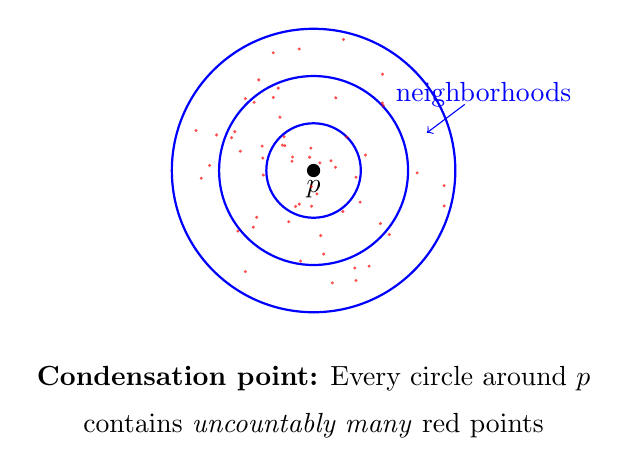
\begin{tikzpicture}[scale=1.2]
    % Draw the point p
    \fill (0,0) circle (2pt) node[below] {$p$};

    % Draw neighborhoods
    \draw[blue, thick] (0,0) circle (1.5);
    \draw[blue, thick] (0,0) circle (1.0);
    \draw[blue, thick] (0,0) circle (0.5);

    % Draw many dots representing uncountably many points
    \foreach \i in {1,...,60} {
        \pgfmathsetmacro{\r}{0.1 + 1.4*rnd}
        \pgfmathsetmacro{\a}{360*rnd}
        \fill[red, opacity=0.7] ({\r*cos(\a)}, {\r*sin(\a)}) circle (0.5pt);
    }

    % Labels
    \node[blue] at (1.8, 0.8) {neighborhoods};
    \draw[->, blue] (1.6, 0.7) -- (1.2, 0.4);

    \node at (0, -2.2) {\textbf{Condensation point:} Every circle around $p$};
    \node at (0, -2.7) {contains \emph{uncountably many} red points};
\end{tikzpicture}
\end{center}

\subsection{Comparison: Limit Point vs Condensation Point}

\begin{center}
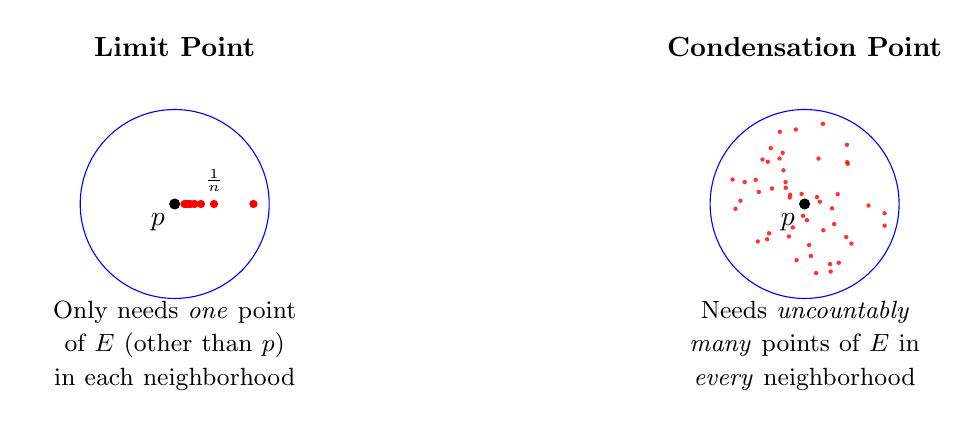
\begin{tikzpicture}[scale=1]
    % LIMIT POINT example
    \begin{scope}[xshift=-4cm]
        \node at (0, 2) {\textbf{Limit Point}};
        \fill (0,0) circle (2pt) node[below left] {$p$};
        \draw[blue] (0,0) circle (1.2);

        % Just a few points (sequence 1/n approaching 0)
        \foreach \n in {1,2,3,4,5,6,7,8} {
            \pgfmathsetmacro{\x}{1.0/\n}
            \fill[red] (\x, 0) circle (1.5pt);
        }
        \node at (0.5, 0.3) {\tiny $\frac{1}{n}$};

        \node[text width=3.5cm, align=center] at (0, -1.8) {\small Only needs \emph{one} point of $E$ (other than $p$) in each neighborhood};
    \end{scope}

    % CONDENSATION POINT example
    \begin{scope}[xshift=4cm]
        \node at (0, 2) {\textbf{Condensation Point}};
        \fill (0,0) circle (2pt) node[below left] {$p$};
        \draw[blue] (0,0) circle (1.2);

        % Many many points
        \foreach \i in {1,...,50} {
            \pgfmathsetmacro{\r}{0.1 + 1.0*rnd}
            \pgfmathsetmacro{\a}{360*rnd}
            \fill[red, opacity=0.8] ({\r*cos(\a)}, {\r*sin(\a)}) circle (0.8pt);
        }

        \node[text width=3.5cm, align=center] at (0, -1.8) {\small Needs \emph{uncountably many} points of $E$ in \emph{every} neighborhood};
    \end{scope}
\end{tikzpicture}
\end{center}

\section{Quick Review: Countable vs Uncountable}

\begin{center}
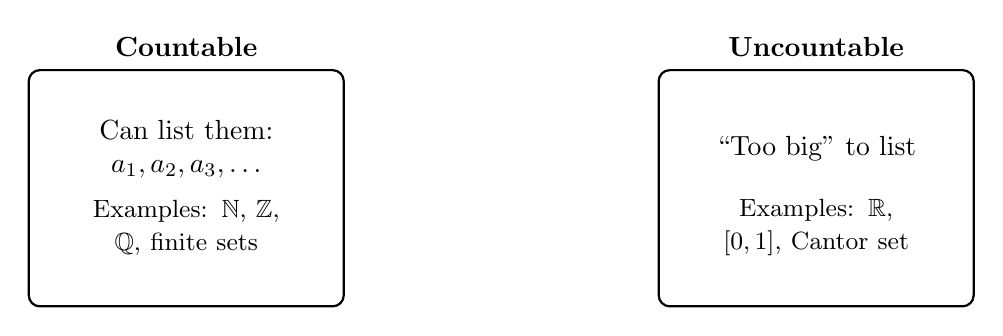
\begin{tikzpicture}
    % Countable
    \begin{scope}[xshift=-4cm]
        \draw[thick, rounded corners] (-2, -1.5) rectangle (2, 1.5);
        \node at (0, 1.8) {\textbf{Countable}};
        \node[text width=3.5cm, align=center] at (0, 0.5) {Can list them: $a_1, a_2, a_3, \ldots$};
        \node[text width=3.5cm, align=center] at (0, -0.5) {\small Examples: $\N$, $\mathbb{Z}$, $\Q$, finite sets};
    \end{scope}

    % Uncountable
    \begin{scope}[xshift=4cm]
        \draw[thick, rounded corners] (-2, -1.5) rectangle (2, 1.5);
        \node at (0, 1.8) {\textbf{Uncountable}};
        \node[text width=3.5cm, align=center] at (0, 0.5) {``Too big'' to list};
        \node[text width=3.5cm, align=center] at (0, -0.5) {\small Examples: $\R$, $[0,1]$, Cantor set};
    \end{scope}
\end{tikzpicture}
\end{center}

\textbf{Key fact:} A countable union of countable sets is countable.

\section{What the Problem Asks}

Given: $E \subset \R^k$ is uncountable.

Define: $P = \{\text{all condensation points of } E\}$.

\textbf{Prove two things:}
\begin{enumerate}
    \item $P$ is \textbf{perfect} (closed + every point is a limit point)
    \item At most countably many points of $E$ are \emph{not} in $P$
\end{enumerate}

\begin{center}
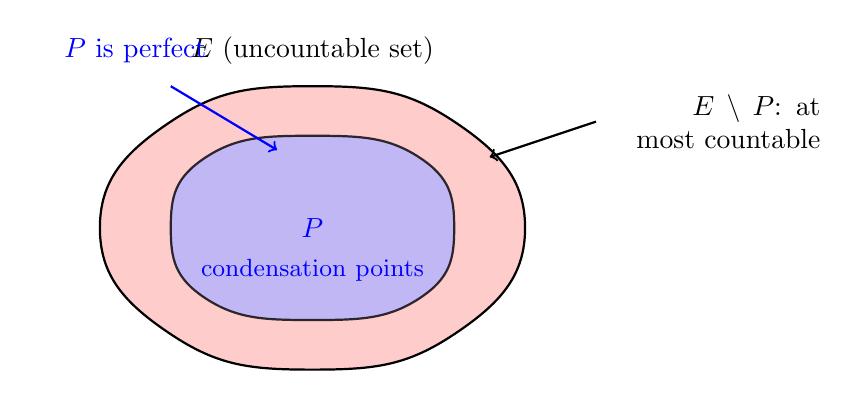
\begin{tikzpicture}[scale=0.9]
    % Draw E as a blob
    \draw[thick, fill=red!20] plot[smooth cycle, tension=0.8] coordinates {(-3,0) (-2,1.5) (0,2) (2,1.5) (3,0) (2,-1.5) (0,-2) (-2,-1.5)};
    \node at (0, 2.5) {$E$ (uncountable set)};

    % Draw P inside
    \draw[thick, fill=blue!30, opacity=0.8] plot[smooth cycle, tension=0.8] coordinates {(-2,0) (-1.5,1) (0,1.3) (1.5,1) (2,0) (1.5,-1) (0,-1.3) (-1.5,-1)};
    \node[blue] at (0, 0) {$P$};
    \node[blue, text width=3cm, align=center] at (0, -0.6) {\small condensation points};

    % Show the ``thin'' part outside P
    \draw[<-, thick] (2.5, 1) -- (4, 1.5);
    \node[text width=3cm, align=right] at (5.5, 1.5) {$E \setminus P$: at most countable};

    % Arrow to P
    \draw[<-, thick, blue] (-0.5, 1.1) -- (-2, 2);
    \node[blue, text width=2.5cm, align=center] at (-2.5, 2.5) {$P$ is perfect};
\end{tikzpicture}
\end{center}

\section{What is a Perfect Set?}

A set $P$ is \textbf{perfect} if:
\begin{enumerate}
    \item $P$ is \textbf{closed} (contains all its limit points), AND
    \item Every point of $P$ is a \textbf{limit point} of $P$ (no isolated points)
\end{enumerate}

\begin{center}
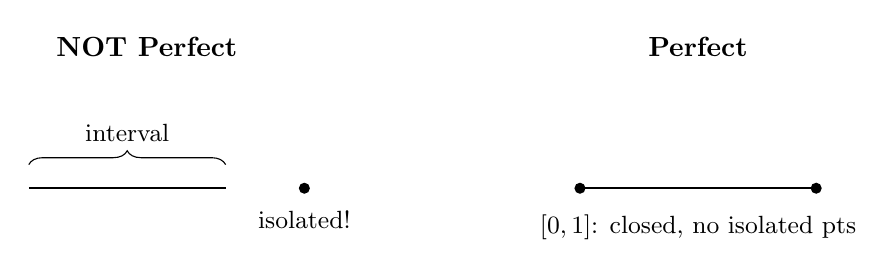
\begin{tikzpicture}[scale=1]
    % NOT perfect - has isolated point
    \begin{scope}[xshift=-4cm]
        \node at (0, 1.8) {\textbf{NOT Perfect}};
        \draw[thick] (-1.5, 0) -- (1, 0);
        \fill (2, 0) circle (2pt);
        \node at (2, -0.4) {\small isolated!};
        \draw[decorate, decoration={brace, amplitude=5pt}] (-1.5, 0.3) -- (1, 0.3);
        \node at (-0.25, 0.7) {\small interval};
    \end{scope}

    % Perfect - like [0,1]
    \begin{scope}[xshift=3cm]
        \node at (0, 1.8) {\textbf{Perfect}};
        \draw[thick] (-1.5, 0) -- (1.5, 0);
        \fill (-1.5, 0) circle (2pt);
        \fill (1.5, 0) circle (2pt);
        \node at (0, -0.5) {\small $[0,1]$: closed, no isolated pts};
    \end{scope}
\end{tikzpicture}
\end{center}

\textbf{Classic example:} The Cantor set is perfect (and uncountable!).

\section{The Hint Explained}

The hint says: Let $\{V_n\}$ be a countable base of $\R^k$...

\subsection{What is a Countable Base?}

A \textbf{base} is a collection of open sets such that every open set is a union of sets from the base.

For $\R^k$: Use open balls with \textbf{rational} centers and \textbf{rational} radii.

\begin{center}
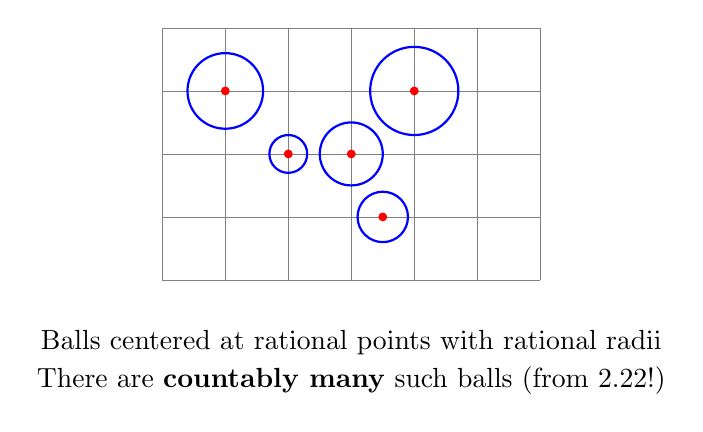
\begin{tikzpicture}[scale=0.8]
    % Grid representing R^2
    \draw[gray, very thin] (-3,-2) grid (3,2);

    % Some balls with rational centers
    \draw[blue, thick] (0,0) circle (0.5);
    \draw[blue, thick] (1,1) circle (0.7);
    \draw[blue, thick] (-1,0) circle (0.3);
    \draw[blue, thick] (0.5,-1) circle (0.4);
    \draw[blue, thick] (-2,1) circle (0.6);

    % Rational points
    \fill[red] (0,0) circle (2pt);
    \fill[red] (1,1) circle (2pt);
    \fill[red] (-1,0) circle (2pt);
    \fill[red] (0.5,-1) circle (2pt);
    \fill[red] (-2,1) circle (2pt);

    \node at (0, -3) {Balls centered at rational points with rational radii};
    \node at (0, -3.6) {There are \textbf{countably many} such balls (from 2.22!)};
\end{tikzpicture}
\end{center}

\subsection{The Strategy}

Define $W = $ union of all $V_n$ where $E \cap V_n$ is countable.

\begin{center}
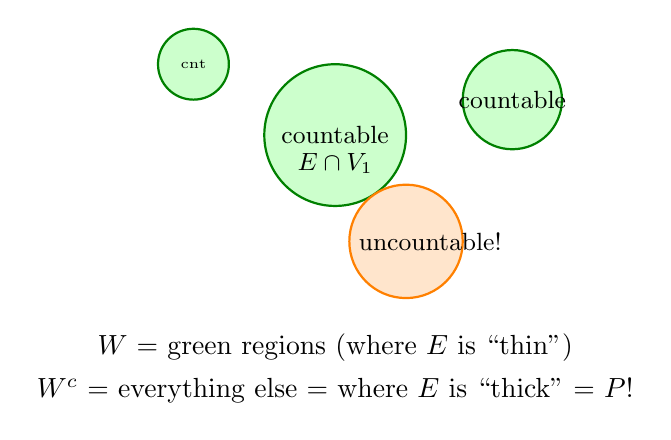
\begin{tikzpicture}[scale=0.9]
    % Show some V_n's
    \draw[green!50!black, thick, fill=green!20] (0,0) circle (1);
    \node at (0,0) {\small countable};
    \node at (0, -0.4) {\small $E \cap V_1$};

    \draw[green!50!black, thick, fill=green!20] (2.5, 0.5) circle (0.7);
    \node at (2.5, 0.5) {\small countable};

    \draw[green!50!black, thick, fill=green!20] (-2, 1) circle (0.5);
    \node at (-2, 1) {\tiny cnt};

    \draw[orange, thick, fill=orange!20] (1, -1.5) circle (0.8);
    \node[text width=1.2cm, align=center] at (1, -1.5) {\small uncountable!};

    \node at (0, -3) {$W$ = green regions (where $E$ is ``thin'')};
    \node at (0, -3.6) {$W^c$ = everything else = where $E$ is ``thick'' = $P$!};
\end{tikzpicture}
\end{center}

\textbf{Key insight:}
\begin{itemize}
    \item $W$ is a countable union of sets, each containing only countably many points of $E$
    \item So $E \cap W$ is countable (countable union of countable sets)
    \item The ``interesting'' points of $E$ (uncountably many) must be in $W^c = P$
\end{itemize}

\section{Summary of the Proof Strategy}

\begin{enumerate}
    \item Show $P = W^c$ (condensation points are exactly the complement of $W$)
    \item $W$ is open (union of open sets), so $P = W^c$ is \textbf{closed}
    \item Show every point of $P$ is a limit point of $P$ (so $P$ is \textbf{perfect})
    \item $E \cap W$ is countable, so $E \setminus P = E \cap W$ is countable
\end{enumerate}

\end{document}
